% !TEX root = ../main.tex
%
\chapter{Proposed adaptive SPS}
\label{solution}
In this chapter, we present our self-adaptive SPS capable of providing high throughput, scalability, and low latency, while guaranteeing the integrity of the results obtained from the analysed data. Our proposal, which is an extension of \textit{Storm}, dynamically adapts the number of operator replicas to cope with environments that present highly variable input rate environments.

This chapter is structured in three sections. Section \ref{modified-sps} presents the extensions made in \textit{Storm} to circumvent its limitations. Then, Section \ref{reactive-approach} presents \rSPS{}, our proposed \textit{reactive approach}, published in \citep{WladdimiroNCA}, which is based on multi-metrics. Finally, Section \ref{predictive-approach} presents \pSPS{}, our \textit{predictive approach}, published in \citep{WladdimiroSBAC}, which focuses on predicting the number of replicas required by for the next time interval.


\section{New features of the adaptive SPS}
\label{modified-sps}
Most SPSs require expert knowledge for configuring the system's processing resources according to the environment requirements. Furthermore, they can not reconfigure themselves at runtime. Highly variable input rate environments may induce resource over-provisioning, wasting processing resources, while under-provisioning, may induce the loss of data processing.

In order to handle such scenarios, \rSPS{} and \pSPS{} can dynamically allocate/deallocate operators' replicas at runtime. Such an elasticity enables the two adaptive SPSs to adapt their processing logic, optimizing resource usage while minimizing data loss.

Both SPSs exploit two mechanisms that do not exist in the original \textit{Storm}: a pool of replicas and a \textit{load-aware} grouping strategy. The first one attempts to reduce adaptation reaction delay reducing, therefore, event processing latency. \textit{Storm}'s original version provides a rebalancing feature to reallocate the number of executors for a bolt. However, this action involves system downtime, loss of messages, and increasing of end-to-end latency which degrades performance. The second mechanism handles operators' replicas event distribution. Grouping strategies in \textit{Storm} define how events are distributed among operators. Due to the heterogeneous nature of the processing resources and operators' tasks complexity, balance issues may occur, creating bottlenecks and increasing latency.

\subsection{Pool of replicas}
\label{pool}

At initialization, \rSPS{} and \pSPS{} assign, for each operator, a pool of replicas deployed by the scheduler. Replicas can be either in  \textit{active} or \textit{inactive} state. The state of a replica can be modified at runtime. An inactive (resp., active) replica consumes negligible (resp., non negligible) CPU power and can be dynamically activated (resp., deactivated) whenever the prediction model of the system detects the need for increasing (resp., decreasing) the replicas for the operator in question. Thus, based on the number of available cores by VMs and the fact that, in general, each replica is associated with a thread, it is possible to set the size of a pool ($p$), which is the same for each operator pool. 

Figure \ref{fig:pool} considers a DAG with operators $O_A$ and $O_B$ and their respective pool of replicas of size $p$. When initialising the application, there is only one active replica per operator as shown in Figure \ref{fig:pool-without} there is only one active replica per operator ($O_{A.1}$ and $O_{B.1}$). Therefore, the other replicas are inactive and do not receive a data stream. It is important to note that it is necessary to keep one replica active, since if all replicas are inactive, the DAG components related to the operator would be lost. The state of an operator can be modified, as is the case of $O_{A.2}$, which changes from inactive to active as shown in Figure \ref{fig:pool-with}. When this is done, the stream data sharing is determined by the grouping strategy of the operator (see Section \ref{grouping}).

\begin{figure}[!ht]
\begin{center}
\subfloat[One active replica per operator.]{
  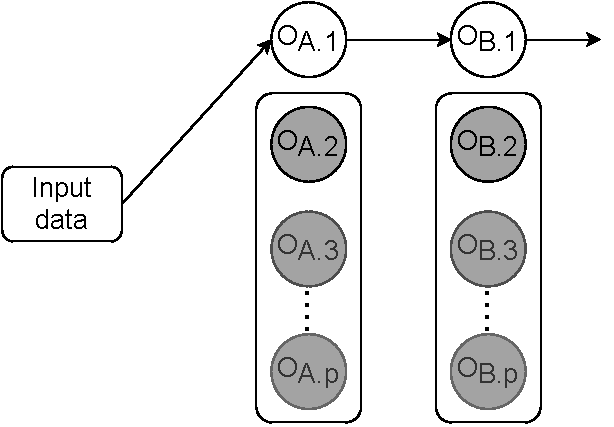
\includegraphics[width=0.5\textwidth]{figures/concepts/ASPS-PoolReplica-1.pdf}
    \label{fig:pool-without}
}
\subfloat[Activation of a replica.]{
	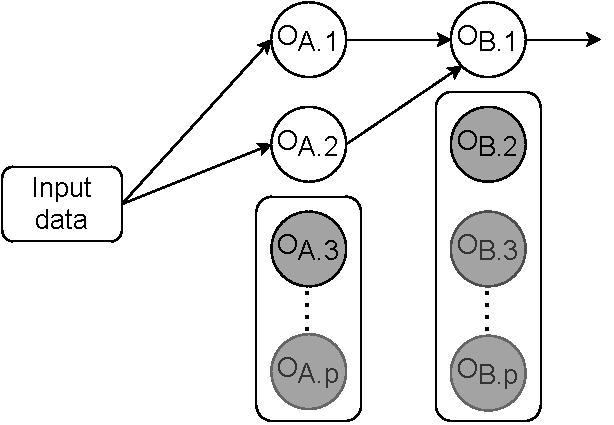
\includegraphics[width=0.5\textwidth]{figures/concepts/ASPS-PoolReplica-2.pdf}
    \label{fig:pool-with}
}
 \caption{Example of pool replicas for two operators.}
    \label{fig:pool}
\end{center}
\end{figure}

Despite its simplicity, performance results showed that the pool of replica is very effective, since \rSPS{} and \pSPS{} are self-adaptive at runtime at a negligible cost. Moreover, as it is implemented in \textit{Storm}, there is no need to restart the application, so downtime is avoided.

\subsection{Load-Aware Grouping}
\label{grouping}
A grouping technique specifies how a stream (tuples) should be partitioned among operators. Using traditional methods like \textit{Shuffle grouping} (see Section \ref{grouping}), tuples are randomly distributed across operators, ensuring that each operator receives an equal number of tuples. Due to the complexity of the tasks or the heterogeneous nature of the processing resources, load balance issues may occur. In this case, while pending events are still in the processing queue, new events can go on arriving. 

To overcome this problem, we propose a \textit{load-aware grouping} strategy, which considers the load state of active replicas in terms of $\mu_{i.j}(t)$, i.e., the number of events processed by replica $j$ of an operator $i$ during a time interval $t$, $et_i$, the average execution time of one event at operator $i$, and $td$, the time interval duration. Note that we define a replica $j$ of an operator $i$ as $O_{i.j}$.

Therefore, the proportional distribution of events considers the current utilization of active replicas. The utilization is computed following Equation \ref{eq:utilization}, where $U$ ranges between $0$ and $1$ for a replica $j$ of an operator $i$. A $0$ and $1$ values represent $0\%$ and $100\%$ utilization of the replica respectively. If all replicas present the same utilization value, events are sent in a round-robin fashion. Otherwise, events will be assigned to the replica with  the lowest load.

\begin{equation}
\label{eq:utilization}
    U_{i.j}(t) = \frac{\mu_{i.j}(t) \times et_i}{td}
\end{equation}

Algorithm \ref{alg:grouping} shows the pseudo-code of the \textit{load-aware grouping} strategy. The loop of lines 3-7 is responsible for selecting the replica $j$ of operator $O_i$ with the lowest utilisation. Then, if the utilisation is $100\%$ ($U=1$), which means that all the replicas are overloaded, a replica candidate is randomly chosen (lines 8-9). Otherwise, the overhead of processing the event is added to the replica candidate utilisation (line 11). Finally in line 13, the event is sent to the replica candidate of the $O_i$ operator.

\begin{algorithm}
\caption{Load-Aware grouping for operator $O_i$.}
\begin{algorithmic}[1]
 	\REQUIRE Statistics of replicas of $O_{i}$ in interval $t$.
 	\ENSURE Replica $O_{i.m}$ that should process the event.
 	\STATE {$m \gets 0$}
 	\STATE {$p \gets$ sizePoolReplicas($O_i$)}
 	\FOR {$j : 1 \to p$}
 	    \IF {$U_{i.j} < U_{i.m}$}
 	        \STATE {$m \gets j$}
 	    \ENDIF
 	\ENDFOR
 	\IF {$U_{i.m} = 1$}
  	    \STATE {$m \gets$ getReplicaRoundRobin($O_{i}$)}
  	\ELSE
  	    \STATE $U_{i.m} \gets U_{i.m} + \frac{et_i}{td}$  
 	\ENDIF
 	\STATE sendEvent($O_{i.m}$)
\end{algorithmic}
\label{alg:grouping}
\end{algorithm}